\documentclass[1p]{elsarticle_modified}
%\bibliographystyle{elsarticle-num}

%\usepackage[colorlinks]{hyperref}
%\usepackage{abbrmath_seonhwa} %\Abb, \Ascr, \Acal ,\Abf, \Afrak
\usepackage{amsfonts}
\usepackage{amssymb}
\usepackage{amsmath}
\usepackage{amsthm}
\usepackage{scalefnt}
\usepackage{amsbsy}
\usepackage{kotex}
\usepackage{caption}
\usepackage{subfig}
\usepackage{color}
\usepackage{graphicx}
\usepackage{xcolor} %% white, black, red, green, blue, cyan, magenta, yellow
\usepackage{float}
\usepackage{setspace}
\usepackage{hyperref}

\usepackage{tikz}
\usetikzlibrary{arrows}

\usepackage{multirow}
\usepackage{array} % fixed length table
\usepackage{hhline}

%%%%%%%%%%%%%%%%%%%%%
\makeatletter
\renewcommand*\env@matrix[1][\arraystretch]{%
	\edef\arraystretch{#1}%
	\hskip -\arraycolsep
	\let\@ifnextchar\new@ifnextchar
	\array{*\c@MaxMatrixCols c}}
\makeatother %https://tex.stackexchange.com/questions/14071/how-can-i-increase-the-line-spacing-in-a-matrix
%%%%%%%%%%%%%%%

\usepackage[normalem]{ulem}

\newcommand{\msout}[1]{\ifmmode\text{\sout{\ensuremath{#1}}}\else\sout{#1}\fi}
%SOURCE: \msout is \stkout macro in https://tex.stackexchange.com/questions/20609/strikeout-in-math-mode

\newcommand{\cancel}[1]{
	\ifmmode
	{\color{red}\msout{#1}}
	\else
	{\color{red}\sout{#1}}
	\fi
}

\newcommand{\add}[1]{
	{\color{blue}\uwave{#1}}
}

\newcommand{\replace}[2]{
	\ifmmode
	{\color{red}\msout{#1}}{\color{blue}\uwave{#2}}
	\else
	{\color{red}\sout{#1}}{\color{blue}\uwave{#2}}
	\fi
}

\newcommand{\Sol}{\mathcal{S}} %segment
\newcommand{\D}{D} %diagram
\newcommand{\A}{\mathcal{A}} %arc


%%%%%%%%%%%%%%%%%%%%%%%%%%%%%5 test

\def\sl{\operatorname{\textup{SL}}(2,\Cbb)}
\def\psl{\operatorname{\textup{PSL}}(2,\Cbb)}
\def\quan{\mkern 1mu \triangleright \mkern 1mu}

\theoremstyle{definition}
\newtheorem{thm}{Theorem}[section]
\newtheorem{prop}[thm]{Proposition}
\newtheorem{lem}[thm]{Lemma}
\newtheorem{ques}[thm]{Question}
\newtheorem{cor}[thm]{Corollary}
\newtheorem{defn}[thm]{Definition}
\newtheorem{exam}[thm]{Example}
\newtheorem{rmk}[thm]{Remark}
\newtheorem{alg}[thm]{Algorithm}

\newcommand{\I}{\sqrt{-1}}
\begin{document}

%\begin{frontmatter}
%
%\title{Boundary parabolic representations of knots up to 8 crossings}
%
%%% Group authors per affiliation:
%\author{Yunhi Cho} 
%\address{Department of Mathematics, University of Seoul, Seoul, Korea}
%\ead{yhcho@uos.ac.kr}
%
%
%\author{Seonhwa Kim} %\fnref{s_kim}}
%\address{Center for Geometry and Physics, Institute for Basic Science, Pohang, 37673, Korea}
%\ead{ryeona17@ibs.re.kr}
%
%\author{Hyuk Kim}
%\address{Department of Mathematical Sciences, Seoul National University, Seoul 08826, Korea}
%\ead{hyukkim@snu.ac.kr}
%
%\author{Seokbeom Yoon}
%\address{Department of Mathematical Sciences, Seoul National University, Seoul, 08826,  Korea}
%\ead{sbyoon15@snu.ac.kr}
%
%\begin{abstract}
%We find all boundary parabolic representation of knots up to 8 crossings.
%
%\end{abstract}
%\begin{keyword}
%    \MSC[2010] 57M25 
%\end{keyword}
%
%\end{frontmatter}

%\linenumbers
%\tableofcontents
%
\newcommand\colored[1]{\textcolor{white}{\rule[-0.35ex]{0.8em}{1.4ex}}\kern-0.8em\color{red} #1}%
%\newcommand\colored[1]{\textcolor{white}{ #1}\kern-2.17ex	\textcolor{white}{ #1}\kern-1.81ex	\textcolor{white}{ #1}\kern-2.15ex\color{red}#1	}

{\Large $\underline{12a_{0596}~(K12a_{0596})}$}

\setlength{\tabcolsep}{10pt}
\renewcommand{\arraystretch}{1.6}
\vspace{1cm}\begin{tabular}{m{100pt}>{\centering\arraybackslash}m{274pt}}
\multirow{5}{120pt}{
	\centering
	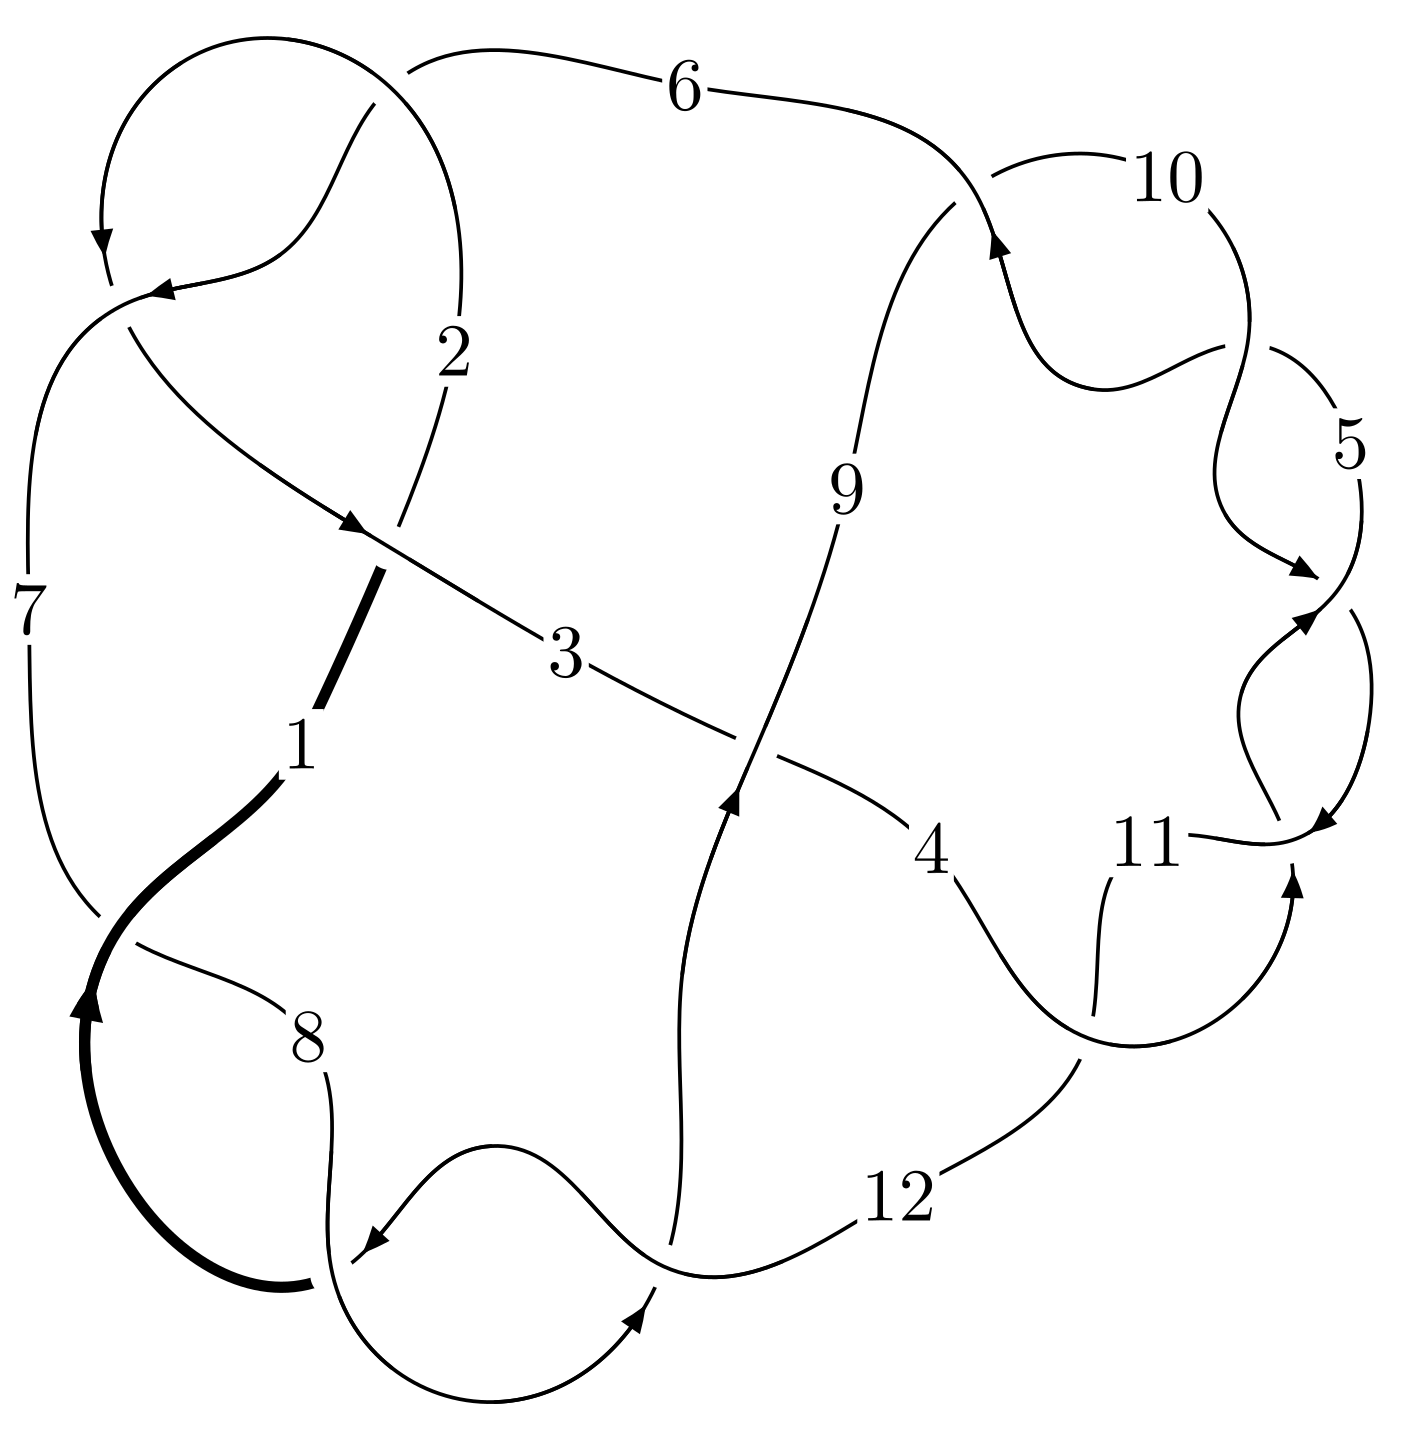
\includegraphics[width=112pt]{../../../GIT/diagram.site/Diagrams/png/1397_12a_0596.png}\\
\ \ \ A knot diagram\footnotemark}&
\allowdisplaybreaks
\textbf{Linearized knot diagam} \\
\cline{2-2}
 &
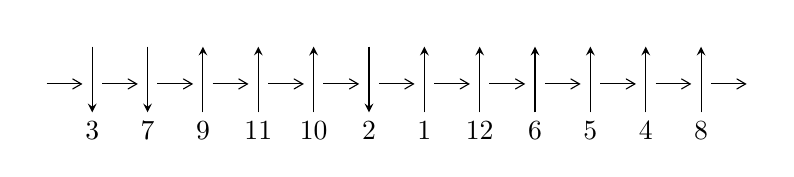
\begin{tikzpicture}[x=20pt, y=17pt]
	% nodes
	\node (C0) at (0, 0) {};
	\node (C1) at (1, 0) {};
	\node (C1U) at (1, +1) {};
	\node (C1D) at (1, -1) {3};

	\node (C2) at (2, 0) {};
	\node (C2U) at (2, +1) {};
	\node (C2D) at (2, -1) {7};

	\node (C3) at (3, 0) {};
	\node (C3U) at (3, +1) {};
	\node (C3D) at (3, -1) {9};

	\node (C4) at (4, 0) {};
	\node (C4U) at (4, +1) {};
	\node (C4D) at (4, -1) {11};

	\node (C5) at (5, 0) {};
	\node (C5U) at (5, +1) {};
	\node (C5D) at (5, -1) {10};

	\node (C6) at (6, 0) {};
	\node (C6U) at (6, +1) {};
	\node (C6D) at (6, -1) {2};

	\node (C7) at (7, 0) {};
	\node (C7U) at (7, +1) {};
	\node (C7D) at (7, -1) {1};

	\node (C8) at (8, 0) {};
	\node (C8U) at (8, +1) {};
	\node (C8D) at (8, -1) {12};

	\node (C9) at (9, 0) {};
	\node (C9U) at (9, +1) {};
	\node (C9D) at (9, -1) {6};

	\node (C10) at (10, 0) {};
	\node (C10U) at (10, +1) {};
	\node (C10D) at (10, -1) {5};

	\node (C11) at (11, 0) {};
	\node (C11U) at (11, +1) {};
	\node (C11D) at (11, -1) {4};

	\node (C12) at (12, 0) {};
	\node (C12U) at (12, +1) {};
	\node (C12D) at (12, -1) {8};
	\node (C13) at (13, 0) {};

	% arrows
	\draw[->,>={angle 60}]
	(C0) edge (C1) (C1) edge (C2) (C2) edge (C3) (C3) edge (C4) (C4) edge (C5) (C5) edge (C6) (C6) edge (C7) (C7) edge (C8) (C8) edge (C9) (C9) edge (C10) (C10) edge (C11) (C11) edge (C12) (C12) edge (C13) ;	\draw[->,>=stealth]
	(C1U) edge (C1D) (C2U) edge (C2D) (C3D) edge (C3U) (C4D) edge (C4U) (C5D) edge (C5U) (C6U) edge (C6D) (C7D) edge (C7U) (C8D) edge (C8U) (C9D) edge (C9U) (C10D) edge (C10U) (C11D) edge (C11U) (C12D) edge (C12U) ;
	\end{tikzpicture} \\
\hhline{~~} \\& 
\textbf{Solving Sequence} \\ \cline{2-2} 
 &
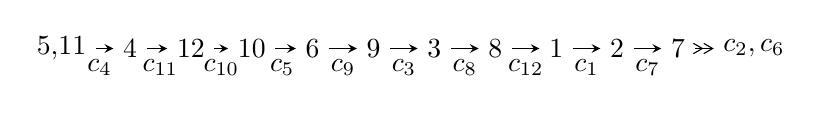
\begin{tikzpicture}[x=22pt, y=7pt]
	% node
	\node (A0) at (-1/8, 0) {5,11};
	\node (A1) at (1, 0) {4};
	\node (A2) at (2, 0) {12};
	\node (A3) at (3, 0) {10};
	\node (A4) at (4, 0) {6};
	\node (A5) at (5, 0) {9};
	\node (A6) at (6, 0) {3};
	\node (A7) at (7, 0) {8};
	\node (A8) at (8, 0) {1};
	\node (A9) at (9, 0) {2};
	\node (A10) at (10, 0) {7};
	\node (C1) at (1/2, -1) {$c_{4}$};
	\node (C2) at (3/2, -1) {$c_{11}$};
	\node (C3) at (5/2, -1) {$c_{10}$};
	\node (C4) at (7/2, -1) {$c_{5}$};
	\node (C5) at (9/2, -1) {$c_{9}$};
	\node (C6) at (11/2, -1) {$c_{3}$};
	\node (C7) at (13/2, -1) {$c_{8}$};
	\node (C8) at (15/2, -1) {$c_{12}$};
	\node (C9) at (17/2, -1) {$c_{1}$};
	\node (C10) at (19/2, -1) {$c_{7}$};
	\node (A11) at (45/4, 0) {$c_{2},c_{6}$};

	% edge
	\draw[->,>=stealth]	
	(A0) edge (A1) (A1) edge (A2) (A2) edge (A3) (A3) edge (A4) (A4) edge (A5) (A5) edge (A6) (A6) edge (A7) (A7) edge (A8) (A8) edge (A9) (A9) edge (A10) ;
	\draw[->>,>={angle 60}]	
	(A10) edge (A11);
\end{tikzpicture} \\ 

\end{tabular} \\

\footnotetext{
The image of knot diagram is generated by the software ``\textbf{Draw programme}" developed by Andrew Bartholomew(\url{http://www.layer8.co.uk/maths/draw/index.htm\#Running-draw}), where we modified some parts for our purpose(\url{https://github.com/CATsTAILs/LinksPainter}).
}\phantom \\ \newline 
\centering \textbf{Ideals for irreducible components\footnotemark of $X_{\text{par}}$} 
 
\begin{align*}
I^u_{1}&=\langle 
u^{40}+u^{39}+\cdots+2 u+1\rangle \\
\\
\end{align*}
\raggedright * 1 irreducible components of $\dim_{\mathbb{C}}=0$, with total 40 representations.\\
\footnotetext{All coefficients of polynomials are rational numbers. But the coefficients are sometimes approximated in decimal forms when there is not enough margin.}
\newpage
\renewcommand{\arraystretch}{1}
\centering \section*{I. $I^u_{1}= \langle u^{40}+u^{39}+\cdots+2 u+1 \rangle$}
\flushleft \textbf{(i) Arc colorings}\\
\begin{tabular}{m{7pt} m{180pt} m{7pt} m{180pt} }
\flushright $a_{5}=$&$\begin{pmatrix}1\\0\end{pmatrix}$ \\
\flushright $a_{11}=$&$\begin{pmatrix}0\\u\end{pmatrix}$ \\
\flushright $a_{4}=$&$\begin{pmatrix}1\\u^2\end{pmatrix}$ \\
\flushright $a_{12}=$&$\begin{pmatrix}u\\u^3+u\end{pmatrix}$ \\
\flushright $a_{10}=$&$\begin{pmatrix}- u\\u\end{pmatrix}$ \\
\flushright $a_{6}=$&$\begin{pmatrix}u^2+1\\- u^2\end{pmatrix}$ \\
\flushright $a_{9}=$&$\begin{pmatrix}- u^3-2 u\\u^3+u\end{pmatrix}$ \\
\flushright $a_{3}=$&$\begin{pmatrix}- u^8-5 u^6-7 u^4-2 u^2+1\\u^8+4 u^6+4 u^4+2 u^2\end{pmatrix}$ \\
\flushright $a_{8}=$&$\begin{pmatrix}- u^7-4 u^5-4 u^3-2 u\\- u^9-5 u^7-7 u^5-2 u^3+u\end{pmatrix}$ \\
\flushright $a_{1}=$&$\begin{pmatrix}u^{13}+8 u^{11}+23 u^9+30 u^7+20 u^5+6 u^3+u\\u^{15}+9 u^{13}+30 u^{11}+45 u^9+28 u^7+2 u^5-2 u^3+u\end{pmatrix}$ \\
\flushright $a_{2}=$&$\begin{pmatrix}- u^{31}-20 u^{29}+\cdots+32 u^5+14 u^3\\u^{31}+19 u^{29}+\cdots-4 u^3+u\end{pmatrix}$ \\
\flushright $a_{7}=$&$\begin{pmatrix}- u^{19}-12 u^{17}+\cdots-7 u^3-2 u\\- u^{21}-13 u^{19}+\cdots-5 u^3+u\end{pmatrix}$\\&\end{tabular}
\flushleft \textbf{(ii) Obstruction class $= -1$}\\~\\
\flushleft \textbf{(iii) Cusp Shapes $= 4 u^{39}+4 u^{38}+\cdots-4 u+10$}\\~\\
\newpage\renewcommand{\arraystretch}{1}
\flushleft \textbf{(iv) u-Polynomials at the component}\newline \\
\begin{tabular}{m{50pt}|m{274pt}}
Crossings & \hspace{64pt}u-Polynomials at each crossing \\
\hline $$\begin{aligned}c_{1}\end{aligned}$$&$\begin{aligned}
&u^{40}+23 u^{39}+\cdots+4 u+1
\end{aligned}$\\
\hline $$\begin{aligned}c_{2},c_{6}\end{aligned}$$&$\begin{aligned}
&u^{40}- u^{39}+\cdots-2 u+1
\end{aligned}$\\
\hline $$\begin{aligned}c_{3}\end{aligned}$$&$\begin{aligned}
&u^{40}- u^{39}+\cdots+754 u+841
\end{aligned}$\\
\hline $$\begin{aligned}c_{4},c_{5},c_{9}\\c_{10},c_{11}\end{aligned}$$&$\begin{aligned}
&u^{40}- u^{39}+\cdots-2 u+1
\end{aligned}$\\
\hline $$\begin{aligned}c_{7},c_{8},c_{12}\end{aligned}$$&$\begin{aligned}
&u^{40}-3 u^{39}+\cdots-21 u+8
\end{aligned}$\\
\hline
\end{tabular}\\~\\
\newpage\renewcommand{\arraystretch}{1}
\flushleft \textbf{(v) Riley Polynomials at the component}\newline \\
\begin{tabular}{m{50pt}|m{274pt}}
Crossings & \hspace{64pt}Riley Polynomials at each crossing \\
\hline $$\begin{aligned}c_{1}\end{aligned}$$&$\begin{aligned}
&y^{40}-11 y^{39}+\cdots+20 y+1
\end{aligned}$\\
\hline $$\begin{aligned}c_{2},c_{6}\end{aligned}$$&$\begin{aligned}
&y^{40}-23 y^{39}+\cdots-4 y+1
\end{aligned}$\\
\hline $$\begin{aligned}c_{3}\end{aligned}$$&$\begin{aligned}
&y^{40}+29 y^{39}+\cdots+9950712 y+707281
\end{aligned}$\\
\hline $$\begin{aligned}c_{4},c_{5},c_{9}\\c_{10},c_{11}\end{aligned}$$&$\begin{aligned}
&y^{40}+53 y^{39}+\cdots-4 y+1
\end{aligned}$\\
\hline $$\begin{aligned}c_{7},c_{8},c_{12}\end{aligned}$$&$\begin{aligned}
&y^{40}+45 y^{39}+\cdots+727 y+64
\end{aligned}$\\
\hline
\end{tabular}\\~\\
\newpage\flushleft \textbf{(vi) Complex Volumes and Cusp Shapes}
$$\begin{array}{c|c|c}  
\text{Solutions to }I^u_{1}& \I (\text{vol} + \sqrt{-1}CS) & \text{Cusp shape}\\
 \hline 
\begin{aligned}
u &= \phantom{-}0.248211 + 0.953098 I\end{aligned}
 & -4.01639 + 6.06670 I & -0.90138 - 8.69429 I \\ \hline\begin{aligned}
u &= \phantom{-}0.248211 - 0.953098 I\end{aligned}
 & -4.01639 - 6.06670 I & -0.90138 + 8.69429 I \\ \hline\begin{aligned}
u &= \phantom{-}0.117192 + 1.023580 I\end{aligned}
 & -5.72072 - 0.02204 I & -5.47578 + 0. I\phantom{ +0.000000I} \\ \hline\begin{aligned}
u &= \phantom{-}0.117192 - 1.023580 I\end{aligned}
 & -5.72072 + 0.02204 I & -5.47578 + 0. I\phantom{ +0.000000I} \\ \hline\begin{aligned}
u &= -0.182685 + 0.912775 I\end{aligned}
 & -2.08526 - 2.08141 I & \phantom{-}2.66146 + 4.19643 I \\ \hline\begin{aligned}
u &= -0.182685 - 0.912775 I\end{aligned}
 & -2.08526 + 2.08141 I & \phantom{-}2.66146 - 4.19643 I \\ \hline\begin{aligned}
u &= \phantom{-}0.283961 + 1.074480 I\end{aligned}
 & -8.88770 + 4.42504 I & \phantom{-0.000000 } 0. - 3.76885 I \\ \hline\begin{aligned}
u &= \phantom{-}0.283961 - 1.074480 I\end{aligned}
 & -8.88770 - 4.42504 I & \phantom{-0.000000 -}0. + 3.76885 I \\ \hline\begin{aligned}
u &= -0.301843 + 1.075410 I\end{aligned}
 & -12.5035 - 9.2934 I & -3.70345 + 6.82215 I \\ \hline\begin{aligned}
u &= -0.301843 - 1.075410 I\end{aligned}
 & -12.5035 + 9.2934 I & -3.70345 - 6.82215 I \\ \hline\begin{aligned}
u &= -0.277115 + 1.093940 I\end{aligned}
 & -12.82410 + 0.19992 I & -4.32816 + 0. I\phantom{ +0.000000I} \\ \hline\begin{aligned}
u &= -0.277115 - 1.093940 I\end{aligned}
 & -12.82410 - 0.19992 I & -4.32816 + 0. I\phantom{ +0.000000I} \\ \hline\begin{aligned}
u &= -0.118741 + 0.767347 I\end{aligned}
 & -1.15473 - 1.71800 I & \phantom{-}3.78782 + 5.33255 I \\ \hline\begin{aligned}
u &= -0.118741 - 0.767347 I\end{aligned}
 & -1.15473 + 1.71800 I & \phantom{-}3.78782 - 5.33255 I \\ \hline\begin{aligned}
u &= -0.524526 + 0.359238 I\end{aligned}
 & -8.27118 + 2.92235 I & \phantom{-}0.018759 + 0.340430 I \\ \hline\begin{aligned}
u &= -0.524526 - 0.359238 I\end{aligned}
 & -8.27118 - 2.92235 I & \phantom{-}0.018759 - 0.340430 I \\ \hline\begin{aligned}
u &= -0.543635 + 0.321474 I\end{aligned}
 & -8.14588 - 6.41600 I & \phantom{-}0.52066 + 6.62008 I \\ \hline\begin{aligned}
u &= -0.543635 - 0.321474 I\end{aligned}
 & -8.14588 + 6.41600 I & \phantom{-}0.52066 - 6.62008 I \\ \hline\begin{aligned}
u &= \phantom{-}0.519024 + 0.331037 I\end{aligned}
 & -4.50292 + 1.69411 I & \phantom{-}3.60459 - 3.64134 I \\ \hline\begin{aligned}
u &= \phantom{-}0.519024 - 0.331037 I\end{aligned}
 & -4.50292 - 1.69411 I & \phantom{-}3.60459 + 3.64134 I \\ \hline\begin{aligned}
u &= \phantom{-}0.453642 + 0.166928 I\end{aligned}
 & -0.58804 + 3.66392 I & \phantom{-}5.56569 - 8.50417 I \\ \hline\begin{aligned}
u &= \phantom{-}0.453642 - 0.166928 I\end{aligned}
 & -0.58804 - 3.66392 I & \phantom{-}5.56569 + 8.50417 I \\ \hline\begin{aligned}
u &= \phantom{-}0.254529 + 0.390325 I\end{aligned}
 & -1.46728 - 1.22301 I & \phantom{-}0.316991 + 0.035733 I \\ \hline\begin{aligned}
u &= \phantom{-}0.254529 - 0.390325 I\end{aligned}
 & -1.46728 + 1.22301 I & \phantom{-}0.316991 - 0.035733 I \\ \hline\begin{aligned}
u &= -0.384789 + 0.059847 I\end{aligned}
 & \phantom{-}0.863513 - 0.154779 I & \phantom{-}12.21167 + 1.48627 I \\ \hline\begin{aligned}
u &= -0.384789 - 0.059847 I\end{aligned}
 & \phantom{-}0.863513 + 0.154779 I & \phantom{-}12.21167 - 1.48627 I \\ \hline\begin{aligned}
u &= -0.01216 + 1.68251 I\end{aligned}
 & -9.97115 - 2.05842 I & \phantom{-0.000000 } 0 \\ \hline\begin{aligned}
u &= -0.01216 - 1.68251 I\end{aligned}
 & -9.97115 + 2.05842 I & \phantom{-0.000000 } 0 \\ \hline\begin{aligned}
u &= -0.03998 + 1.70308 I\end{aligned}
 & -11.41770 - 2.91186 I & \phantom{-0.000000 } 0 \\ \hline\begin{aligned}
u &= -0.03998 - 1.70308 I\end{aligned}
 & -11.41770 + 2.91186 I & \phantom{-0.000000 } 0\\
 \hline 
 \end{array}$$\newpage$$\begin{array}{c|c|c}  
\text{Solutions to }I^u_{1}& \I (\text{vol} + \sqrt{-1}CS) & \text{Cusp shape}\\
 \hline 
\begin{aligned}
u &= \phantom{-}0.05707 + 1.70742 I\end{aligned}
 & -13.4627 + 7.2396 I & \phantom{-0.000000 } 0 \\ \hline\begin{aligned}
u &= \phantom{-}0.05707 - 1.70742 I\end{aligned}
 & -13.4627 - 7.2396 I & \phantom{-0.000000 } 0 \\ \hline\begin{aligned}
u &= \phantom{-}0.02782 + 1.72703 I\end{aligned}
 & -15.5783 + 0.5569 I & \phantom{-0.000000 } 0 \\ \hline\begin{aligned}
u &= \phantom{-}0.02782 - 1.72703 I\end{aligned}
 & -15.5783 - 0.5569 I & \phantom{-0.000000 } 0 \\ \hline\begin{aligned}
u &= \phantom{-}0.07357 + 1.74076 I\end{aligned}
 & -18.9466 + 5.9094 I & \phantom{-0.000000 } 0 \\ \hline\begin{aligned}
u &= \phantom{-}0.07357 - 1.74076 I\end{aligned}
 & -18.9466 - 5.9094 I & \phantom{-0.000000 } 0 \\ \hline\begin{aligned}
u &= -0.07874 + 1.74141 I\end{aligned}
 & \phantom{-}16.9187 - 10.8760 I & \phantom{-0.000000 } 0 \\ \hline\begin{aligned}
u &= -0.07874 - 1.74141 I\end{aligned}
 & \phantom{-}16.9187 + 10.8760 I & \phantom{-0.000000 } 0 \\ \hline\begin{aligned}
u &= -0.07081 + 1.74611 I\end{aligned}
 & \phantom{-}16.4862 - 1.2511 I & \phantom{-0.000000 } 0 \\ \hline\begin{aligned}
u &= -0.07081 - 1.74611 I\end{aligned}
 & \phantom{-}16.4862 + 1.2511 I & \phantom{-0.000000 } 0\\
 \hline 
 \end{array}$$\newpage
\newpage\renewcommand{\arraystretch}{1}
\centering \section*{ II. u-Polynomials}
\begin{tabular}{m{50pt}|m{274pt}}
Crossings & \hspace{64pt}u-Polynomials at each crossing \\
\hline $$\begin{aligned}c_{1}\end{aligned}$$&$\begin{aligned}
&u^{40}+23 u^{39}+\cdots+4 u+1
\end{aligned}$\\
\hline $$\begin{aligned}c_{2},c_{6}\end{aligned}$$&$\begin{aligned}
&u^{40}- u^{39}+\cdots-2 u+1
\end{aligned}$\\
\hline $$\begin{aligned}c_{3}\end{aligned}$$&$\begin{aligned}
&u^{40}- u^{39}+\cdots+754 u+841
\end{aligned}$\\
\hline $$\begin{aligned}c_{4},c_{5},c_{9}\\c_{10},c_{11}\end{aligned}$$&$\begin{aligned}
&u^{40}- u^{39}+\cdots-2 u+1
\end{aligned}$\\
\hline $$\begin{aligned}c_{7},c_{8},c_{12}\end{aligned}$$&$\begin{aligned}
&u^{40}-3 u^{39}+\cdots-21 u+8
\end{aligned}$\\
\hline
\end{tabular}\newpage\renewcommand{\arraystretch}{1}
\centering \section*{ III. Riley Polynomials}
\begin{tabular}{m{50pt}|m{274pt}}
Crossings & \hspace{64pt}Riley Polynomials at each crossing \\
\hline $$\begin{aligned}c_{1}\end{aligned}$$&$\begin{aligned}
&y^{40}-11 y^{39}+\cdots+20 y+1
\end{aligned}$\\
\hline $$\begin{aligned}c_{2},c_{6}\end{aligned}$$&$\begin{aligned}
&y^{40}-23 y^{39}+\cdots-4 y+1
\end{aligned}$\\
\hline $$\begin{aligned}c_{3}\end{aligned}$$&$\begin{aligned}
&y^{40}+29 y^{39}+\cdots+9950712 y+707281
\end{aligned}$\\
\hline $$\begin{aligned}c_{4},c_{5},c_{9}\\c_{10},c_{11}\end{aligned}$$&$\begin{aligned}
&y^{40}+53 y^{39}+\cdots-4 y+1
\end{aligned}$\\
\hline $$\begin{aligned}c_{7},c_{8},c_{12}\end{aligned}$$&$\begin{aligned}
&y^{40}+45 y^{39}+\cdots+727 y+64
\end{aligned}$\\
\hline
\end{tabular}
\vskip 2pc
\end{document}